%! Licence = CC BY-NC-SA 4.0

%! Author = mariuszindel
%! Date = 12. Jan 2022
%! Project = cydef_summary

\section{MITRE}
\subsection{Cyber Kill Chain}
\begin{center}
    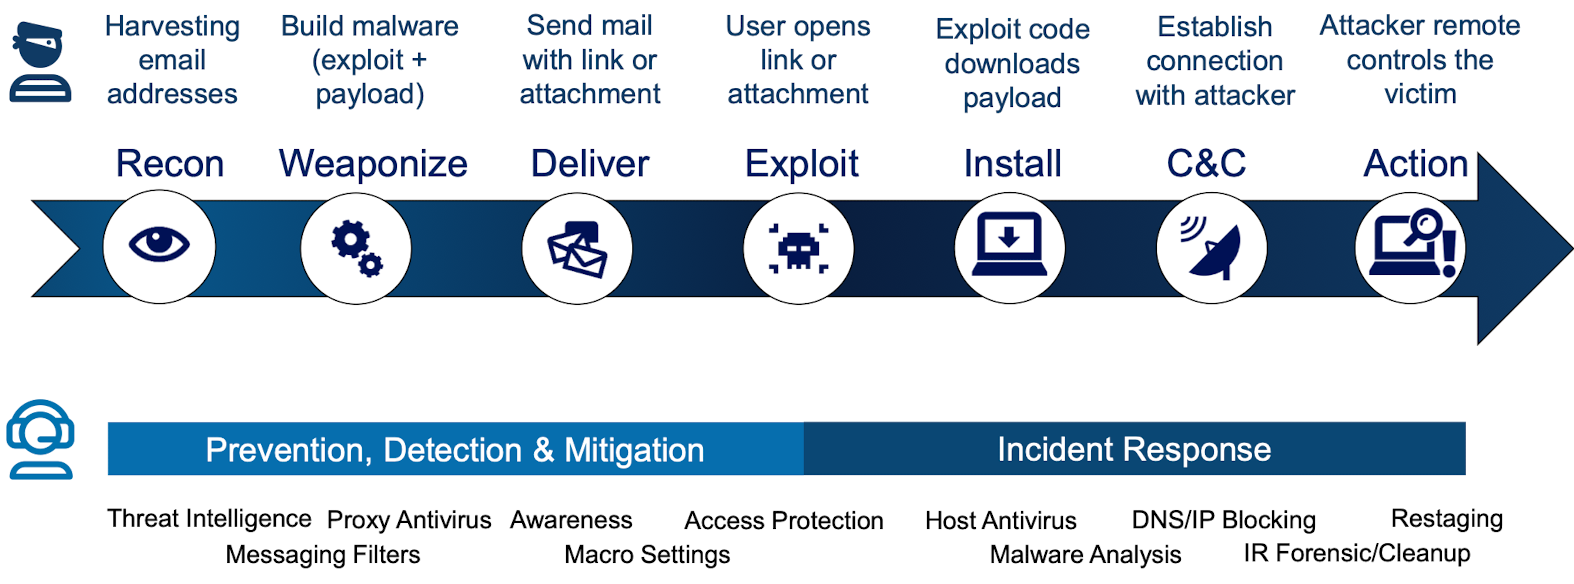
\includegraphics[width=1.0\linewidth]{cyber_kill_chain}
    \vspace{-8pt}
\end{center}


\subsection{MITRE}
\subsubsection{Was ist MITRE ATT\&CK Framework}
\begin{itemize}
    \item Verfolgung der Aktivitäten von mehr als 100 Bedrohungsakteuren (Gruppen)
    \item Sammlung von echten Angriffen
    \item Strukturierte Beobachtungen Technische Details, Anleitungen und Beispiele
    \item Nur Open Source Intelligence
\end{itemize}

\subsubsection{Zweck}
\begin{itemize}
    \item Defenders:
    \begin{itemize}
        \item Bekanntermassen schlechter
        \item Erfassungsgrad der Überwachung
        \item Wirksamkeit der Überwachung
    \end{itemize}
    \item Attackers:
    \begin{itemize}
        \item Ideen für Alternativen
        \item Vermeiden von Fallen
        \item Simulation (Red Teaming)
    \end{itemize}
\end{itemize}

\subsubsection{Heatmap}
Hebt das Spektrum des Erfassungsbereichs hervor, einschliesslich der blinden Flecken (kein Erfassungsbereich)